\documentclass[11pt,a4paper]{article}
\usepackage[utf8]{inputenc}
\usepackage[T1]{fontenc}
\usepackage[french]{babel}
\usepackage{lmodern}
\usepackage{amsmath,amssymb}
\usepackage{bm}
\usepackage{booktabs,array}
\usepackage{graphicx}
\usepackage{tikz}
\usepackage[margin=2.5cm]{geometry}
\usepackage{hyperref}

\newcommand{\vm}{\bm{m}}
\newcommand{\vp}{\bm{p}}
\newcommand{\vs}{\bm{s}}
\newcommand{\vu}{\bm{u}}
\newcommand{\vphi}{\bm{\varphi}}
\newcommand{\Id}{\mathsf{I}}
\newcommand{\mK}{\mathsf{K}}
\newcommand{\ee}{\mathrm{e}}
\emergencystretch=3em

\title{Injection de spin à travers un empilement polariseur :\\
  cas test angulaire sur une couche libre mince}
\author{}
\date{\today}

\begin{document}

\maketitle

\begin{abstract}
  Ce document accompagne le cas de validation
  \texttt{validation/slonczewski\_angle} de la branche \texttt{slonczewski}
  de FeeLLGood. C'est le pendant non colinéaire de
  \texttt{validation/valet\_fert\_1d} : l'aimantation du polariseur fait un
  angle $\theta$ avec celle de la couche libre, le courant de spin
  transverse agit, et la conductance de mélange de la théorie des circuits
  intervient. Le document explique la physique (couple de transfert de
  spin, conductance de mélange, absorption du courant de spin transverse
  sur la longueur s--d), les deux modèles du courant de spin transverse à
  travers l'interface N/F2 proposés par FeeLLGood, la solution de
  référence et les résultats attendus. Dans une limite, le couple
  damping-like a une forme fermée qui montre pourquoi il ne suit
  qu'approximativement la formule de Slonczewski.
\end{abstract}

\tableofcontents

\section{Objet du test}

Dans la branche \texttt{slonczewski}, le polariseur F1, l'espaceur N et les
interfaces F1/N et N/F2 ne sont pas maillés : ils sont remplacés par une
condition de Robin sur la surface d'entrée de la couche libre F2 (clé
\texttt{slonczewski} d'une région de surface,
\texttt{src/slonczewskiInterface.h},
\texttt{spinAcc::stackBoundaryCondition}). Le test colinéaire
\texttt{valet\_fert\_1d} vérifie la partie longitudinale de cette
condition. Ce test-ci vérifie sa partie transverse, celle qui produit le
couple de transfert de spin :
\begin{itemize}
  \item la conversion de la conductance de mélange $G_{\uparrow\downarrow}$
    de la littérature (en S/m$^2$) en conductances du problème de
    diffusion de spin, $G_r + iG_i = 2k\,G_{\uparrow\downarrow}$ ;
  \item le signe du terme en $\mathrm{Im}\,G_{\uparrow\downarrow}$ ;
  \item les deux modèles du courant de spin transverse à travers N/F2,
    \texttt{sink} (par défaut) et \texttt{series} ;
  \item le couplage entre la condition aux limites et la diffusion de spin
    non colinéaire dans F2 (précession, déphasage).
\end{itemize}
La référence est écrite indépendamment de FeeLLGood : la théorie des
circuits de Brataas, Bauer et Kelly pour les interfaces, les équations de
FeeLLGood résolues exactement dans F2.

\section{Rappels physiques}

\subsection{Couple de transfert de spin dans une couche mince}

Un courant qui traverse un ferromagnétique F1 se polarise en spin selon
son aimantation $\vp$. Quand il entre dans un second ferromagnétique F2
d'aimantation $\vm\neq\pm\vp$, la composante de son spin transverse à $\vm$
n'y est pas un état propre : elle précesse autour du champ d'échange et se
déphase en quelques ångströms à un nanomètre. Le moment cinétique qu'elle
perd est transféré à l'aimantation de F2 : c'est le \emph{couple de
transfert de spin}. Il a deux composantes,
\begin{equation}
  \bm{\tau} = \tau_{\mathrm{DL}}\,\vm\times(\vm\times\vp)
            + \tau_{\mathrm{FL}}\,\vm\times\vp ,
\end{equation}
le couple \emph{damping-like}, qui peut compenser l'amortissement et
retourner l'aimantation, et le couple \emph{field-like}, qui agit comme un
champ magnétique selon $\vp$. Slonczewski (1996, 2002) a trouvé pour le
couple damping-like d'une tricouche symétrique la dépendance angulaire
\begin{equation}
  \tau_{\mathrm{DL}} \propto \varepsilon(\theta)\sin\theta,
  \qquad
  \varepsilon(\theta) = \frac{C}{(\Lambda^2+1)+(\Lambda^2-1)\cos\theta},
  \label{eq:slonczewski}
\end{equation}
$\cos\theta = \vm\cdot\vp$. Pour $\Lambda > 1$, le couple est plus grand
près de la configuration antiparallèle ; pour $\Lambda < 1$, près de la
configuration parallèle.

Dans FeeLLGood, le couple sur l'aimantation est proportionnel à
$\vm\times\vs$, où $\vs$ est l'accumulation de spin (en A/m), solution du
problème de diffusion de spin. Avec $\vm = \hat z$ et $\vp$ dans le plan
$(x,z)$, $\vm\times\vp$ est selon $y$ et $\vm\times(\vm\times\vp)$ selon
$-x$ : la composante $s_y$ donne le couple damping-like (puisque
$\vm\times\hat y = -\hat x$) et $s_x$ le couple field-like.

\subsection{Conductance de mélange}

Dans la théorie des circuits de Brataas, Bauer et Kelly, une interface
entre un métal normal N et un ferromagnétique F d'aimantation $\vu$ est
décrite par ses conductances. Pour les composantes de spin selon $\vu$,
les électrons majoritaires ($\uparrow$) et minoritaires ($\downarrow$)
conduisent indépendamment, avec les conductances $G_\uparrow$,
$G_\downarrow$ : c'est le modèle colinéaire de Valet et Fert. Pour les
composantes transverses à $\vu$ apparaît une nouvelle conductance, la
\emph{conductance de mélange}
\begin{equation}
  G_{\uparrow\downarrow} = \frac{e^2}{h}\sum_{n}\Big[1 - \sum_m
    r_\uparrow^{nm}\big(r_\downarrow^{nm}\big)^*\Big]
  = G_r + iG_i \quad\text{(par unité de surface)},
\end{equation}
où $r_{\uparrow(\downarrow)}^{nm}$ sont les amplitudes de réflexion, côté
N, des électrons majoritaires (minoritaires) du canal $m$ vers le canal
$n$. Un spin transverse est une superposition cohérente de $\uparrow$ et
$\downarrow$ ; après réflexion, les deux composantes ont pris des
amplitudes et des phases différentes. Seul le recouvrement $r_\uparrow
r_\downarrow^*$ survit comme spin transverse dans N ; le reste a été
absorbé par F :
\begin{itemize}
  \item $\mathrm{Re}\,G_{\uparrow\downarrow}$ mesure le spin transverse
    absorbé : il produit le couple damping-like ;
  \item $\mathrm{Im}\,G_{\uparrow\downarrow}$ mesure la rotation du spin
    transverse réfléchi autour de $\vu$ : il produit un couple field-like.
\end{itemize}
Pour des interfaces métalliques, $\mathrm{Im}\,G_{\uparrow\downarrow}$ vaut
en général quelques pour cent de $\mathrm{Re}\,G_{\uparrow\downarrow}$ ;
il est ici délibérément grand pour que son signe compte.

\subsection{La loi d'interface}

On utilise les variables de Valet--Fert : $j$ est la densité de courant de
charge selon $+z$, $\vphi = \bm{\mu}_s/e$ l'accumulation de spin en volts
($\mu_s = (\mu_+-\mu_-)/2$ selon l'aimantation, $+$ = majoritaire), et
$\bm{j}_s$ le courant de spin exprimé comme un courant de charge. Le
courant de spin de la gauche (L) vers la droite (R) d'une interface
d'aimantation $\vu$ est
\begin{equation}
  \boxed{\;\bm{j}_s = \gamma\,j\,\vu + \mK(\vu)\,\Delta\vphi,
  \qquad
  \mK(\vu) = \frac{\vu\vu^{\mathsf{T}}}{AR^*}
    + 2G_r\left(\Id-\vu\vu^{\mathsf{T}}\right)
    + 2G_i\,[\,\cdot\times\vu\,]\;}
  \label{eq:interface}
\end{equation}
avec $\Delta\vphi = \vphi_R-\vphi_L$ et $[\,\cdot\times\vu\,]$ la matrice
$\bm{w}\mapsto\bm{w}\times\vu$. Selon $\vu$, c'est la loi de Valet--Fert,
$j_s = \gamma j + \Delta\varphi/AR^*$, avec la résistance d'interface
$AR^*$ et l'asymétrie $\gamma$. Transversalement à $\vu$, c'est l'équation
de Brataas et al.\ pour le courant de spin transverse de N vers F,
$2G_r\,\vm\times(\bm{V}_S\times\vm) + 2G_i\,\bm{V}_S\times\vm$, avec
$\bm{V}_S = -\vphi$ ($\mu = -eV$).

\paragraph{Le facteur 2.} Pour une interface non magnétique ($\gamma = 0$,
$G_\uparrow = G_\downarrow = G_{\uparrow\downarrow} = G$ réel), rien ne
distingue les directions de spin : la conductance doit être isotrope. La
conductance longitudinale vaut $1/AR^* = G_\uparrow+G_\downarrow = 2G$ ; la
conductance transverse doit donc valoir $2G_{\uparrow\downarrow}$. C'est
l'origine du facteur 2 de \eqref{eq:interface}, et de la conversion
$G_r + iG_i = 2k\,G_{\uparrow\downarrow}$ de FeeLLGood
(section~\ref{sec:feellgood}).

\paragraph{Le signe de $\mathrm{Im}\,G_{\uparrow\downarrow}$.} Il se
déduit d'un seul canal. Un spin selon $x$, $(|{\uparrow}\rangle +
|{\downarrow}\rangle)/\sqrt2$, est réfléchi en
$(r_\uparrow|{\uparrow}\rangle + r_\downarrow|{\downarrow}\rangle)/\sqrt2$,
dont la polarisation transverse vaut $r_\uparrow^*r_\downarrow$ (comme
$\langle\sigma_x\rangle + i\langle\sigma_y\rangle$). La polarisation
transverse absorbée vaut $1 - r_\uparrow^*r_\downarrow =
\overline{G_{\uparrow\downarrow}}$ (par canal, en unités de $e^2/h$) : sa
partie imaginaire est $-G_i$, ce qui fixe le signe du dernier terme de
\eqref{eq:interface}. Le test vérifie que le signe opposé échoue.

\subsection{Diffusion de spin dans la couche libre}

Dans F2, FeeLLGood résout
\begin{equation}
  \nabla\cdot Q = -\frac{\vs}{\tau_{sf}} - \frac{\vs\times\vm}{\tau_{sd}},
  \qquad
  Q_{i\alpha} = -P\,\frac{\mu_B}{e}\,j_i\,m_\alpha
  - D_0\left[\partial_i s_\alpha - P^2 m_\alpha(\vm\cdot\partial_i\vs)\right],
  \label{eq:zlf}
\end{equation}
avec $D_0 = 2\sigma/(e^2N_0)$, $1/\tau_{sf} = D_0(1-P^2)/l_{sf}^2$ et
$1/\tau_{sd} = D_0/l_{sd}^2$ ; les indices latins désignent l'espace, les
indices grecs le spin. À une dimension, avec $\vm = \hat z$ uniforme, les
composantes longitudinale et transverses se découplent :
\begin{itemize}
  \item $s_z$ : diffusion $D_0(1-P^2)$, relaxation sur $l_{sf}$, comme
    chez Valet--Fert ;
  \item $\psi = s_x + i s_y$ : diffusion $D_0$ (non réduite), et
    $\vs\times\vm$ devient $-i\psi$, de sorte que
    \begin{equation}
      \psi'' = \kappa^2\,\psi,
      \qquad
      \kappa^2 = \frac{1-P^2}{l_{sf}^2} - \frac{i}{l_{sd}^2} .
    \end{equation}
\end{itemize}
Avec les paramètres du test, $\kappa = (0.718 - 0.697\,i)$\,nm$^{-1}$ :
l'accumulation transverse décroît sur $1/\mathrm{Re}\,\kappa = 1.39$\,nm en
tournant (longueur d'onde $2\pi/|\mathrm{Im}\,\kappa| = 9.0$\,nm). Le
courant de spin qui entre dans F2 polarisé selon $x$ précesse vers $y$ :
c'est pourquoi $s_y$, donc le couple damping-like, apparaît dans F2 même
quand $G_i = 0$, et pourquoi $s_x$ change de signe dans l'épaisseur
(figure~\ref{fig:profil}).

\paragraph{Couple et courant de spin absorbé.} En intégrant la composante
$x$ de \eqref{eq:zlf} sur l'épaisseur $t_2$ ($(\vs\times\vm)_x = s_y$) :
\begin{equation}
  \frac{D_0}{l_{sd}^2}\int_0^{t_2} s_y\,dz
  = q_x(0) - q_x(t_2) - \frac{D_0(1-P^2)}{l_{sf}^2}\int_0^{t_2}s_x\,dz ,
\end{equation}
où $q_x = Q_{zx}$ est le flux de la composante $x$ du moment selon $z$.
L'intégrale de $s_y$, qui mesure le couple damping-like, est le courant de
spin transverse absorbé dans la couche : le courant qui entre, moins celui
qui sort par la sortie et celui que relaxe le renversement de spin. À
$\theta = 90^\circ$ (\texttt{sink}), les trois termes valent $17.15$,
$-1.91$ et $0.14\times10^6$ (unités de $\vs$ fois m/s) : le courant
d'entrée domine.

\subsection{Courant de spin transverse à travers N/F2 : \texttt{sink} ou \texttt{series}}

La théorie des circuits traite le ferromagnétique comme un nœud dont
l'accumulation de spin transverse est nulle : le courant de spin
transverse à travers N/F2 ne dépend que de l'accumulation de l'espaceur.
FeeLLGood, lui, calcule aussi l'accumulation transverse de F2 près de
l'interface. Deux modèles sont proposés (clé \texttt{transverse} de
\texttt{NF2}) :
\begin{itemize}
  \item \texttt{sink} (par défaut) : le courant de spin transverse à
    travers N/F2 ne dépend que de $\vphi_N$, comme en théorie des
    circuits. Dans \eqref{eq:interface}, $\vphi_F$ est remplacé par sa
    partie longitudinale $\vm(\vm\cdot\vphi_F)$. $G_{\uparrow\downarrow}$
    décrit toute l'absorption, et la diffusion dans F2 ne fait que répartir
    le courant absorbé sur $l_{sd}$.
  \item \texttt{series} : il dépend de $\vphi_N - \vphi_F$. L'interface
    ($1/G_{r2}$) et le volume de F2 ($1/g_\perp$, $g_\perp = D_0\kappa$)
    sont alors deux résistances d'absorption en série, et
    $G_{\uparrow\downarrow}$ devrait être la seule part de l'interface
    (Petitjean, Luc et Waintal, 2012). Avec un $G_{\uparrow\downarrow}$
    \emph{ab initio}, qui contient déjà toute l'absorption, celle-ci est
    comptée deux fois.
\end{itemize}
Ici $|2kG_{\uparrow\downarrow}| = 0.70\times10^6$\,m/s et $|g_\perp| =
2.32\times10^6$\,m/s : le volume de F2 ajoute une résistance d'environ un
tiers de celle de l'interface, et le couple damping-like est de 15 à
17\,\% plus petit avec \texttt{series}. La référence suit les deux
modèles.

\section{Le cas test}

\subsection{Géométrie et paramètres}

\begin{figure}[h]
\centering
\begin{tikzpicture}[x=1cm,y=1cm]
  \fill[blue!12] (0,0) rectangle (2.5,1.4);
  \fill[gray!25] (2.5,0) rectangle (2.75,1.4);
  \fill[red!10] (2.75,0) rectangle (8.5,1.4);
  \draw (0,0) rectangle (8.5,1.4);
  \draw[thick] (2.5,0) -- (2.5,1.4);
  \draw[thick] (2.75,0) -- (2.75,1.4);
  \node at (1.25,0.95) {F1};
  \node at (1.25,0.45) {\small réservoir};
  \node at (5.6,0.95) {F2 (maillé, $t_2 = 3$\,nm)};
  \node at (5.6,0.45) {$P$, $l_{sf}$, $l_{sd}$};
  \draw[dashed] (0.7,1.8) -- ++(0:1.0);
  \draw[->,thick] (0.7,1.8) -- ++(35:1.0) node[right] {$\vp$};
  \draw (1.3,1.8) arc (0:35:0.6);
  \node at (1.55,2.0) {\small $\theta$};
  \draw[->,thick] (5.0,1.8) -- ++(0:1.0) node[right] {$\vm = \hat z$};
  \node[below] at (2.6,0) {$z=0$};
  \node[below] at (8.5,0) {$z=t_2$};
  \node[above] at (2.62,1.4) {\small N};
  \draw[<-] (2.45,-0.75) -- (1.8,-1.2) node[left] {\small F1/N};
  \draw[<-] (2.8,-0.75) -- (3.5,-1.2) node[right] {\small N/F2};
  \node[right] at (8.5,0.7) {\small réservoir};
  \draw[->,very thick] (4.2,-0.45) -- (6.2,-0.45) node[right] {\small électrons};
\end{tikzpicture}
\caption{L'empilement. Seul F2 est maillé. Le courant circule selon $z$,
  l'aimantation de F1 est $\vp = (\sin\theta, 0, \cos\theta)$.}
\label{fig:empilement}
\end{figure}

L'empilement est F1 (réservoir idéal, $\vphi = 0$) / F1/N / espaceur N
d'épaisseur nulle / N/F2 / F2 / réservoir ($\vs = 0$),
figure~\ref{fig:empilement}. F2 est une couche de $2\times2$\,nm$^2$ et
d'épaisseur $t_2 = 3$\,nm (\texttt{thin\_layer.geo}, taille de maille
$h = 0.2$\,nm, 1\,695 nœuds, tétraèdres P1), qui résout $l_{sd} = 1$\,nm.
Ses faces latérales ne laissent passer ni charge ni spin : le problème est
unidimensionnel. L'aimantation de F2 est $\vm = \hat z$, celle de F1 est
$\vp = (\sin\theta, 0, \cos\theta)$, $\theta = 0, 30, \dots, 180^\circ$.

\begin{center}
\renewcommand{\arraystretch}{1.2}
\begin{tabular}{llll}
  \toprule
  Élément & Paramètre & Valeur & Clé FeeLLGood \\
  \midrule
  F2 & $\sigma$ & $4\times10^6$\,S/m & \texttt{sigma} \\
    & $P$ & 0.5 & \texttt{P} \\
    & $l_{sf}$, $l_{sd}$ & 5\,nm, 1\,nm & \texttt{l\_sf}, \texttt{l\_sd} \\
    & $N_0$ & $1.344\times10^{47}$\,J$^{-1}$m$^{-3}$ & \texttt{dens\_state} \\
  F1/N & $AR^*$, $\gamma$ & $0.5\times10^{-15}\,\Omega\,$m$^2$, 0.75
    & \texttt{F1N.AR}, \texttt{F1N.gamma} \\
    & $G_{\uparrow\downarrow}$ & $(0.55 + 0.15\,i)\times10^{15}$\,S/m$^2$
    & \texttt{F1N.Gr}, \texttt{F1N.Gi} \\
  N/F2 & $AR^*$, $\gamma$ & $0.5\times10^{-15}\,\Omega\,$m$^2$, 0.75
    & \texttt{NF2.AR}, \texttt{NF2.gamma} \\
    & $G_{\uparrow\downarrow}$ & $(0.55 + 0.25\,i)\times10^{15}$\,S/m$^2$
    & \texttt{NF2.Gr}, \texttt{NF2.Gi} \\
    & modèle & \texttt{sink} ou \texttt{series} & \texttt{NF2.transverse} \\
  Courant & $j_n$ & $10^{12}$\,A/m$^2$ & \texttt{jn} (entrée) \\
  \bottomrule
\end{tabular}
\end{center}
F1 est un réservoir idéal : son volume n'est pas donné (pas de clé
\texttt{F1}), il n'y a pas de renormalisation. Comme dans
\texttt{valet\_fert\_1d}, $j_n > 0$ sur l'entrée (normale sortante $-z$)
signifie que les électrons vont de F1 vers F2, et $j = -j_n$.

\section{Solution de référence}

\subsection{Le système linéaire}

Dans F2, la solution de \eqref{eq:zlf} avec $\vs(t_2) = 0$ est une
combinaison des trois modes propres de
$\left[D_0(\Id - P^2\vm\vm^{\mathsf{T}})\right]^{-1}
\left[D_0(1-P^2)/l_{sf}^2\,\Id + D_0/l_{sd}^2\,[\,\cdot\times\vm\,]\right]$,
de valeurs propres $1/l_{sf}^2$ et $\kappa^2$, $\bar\kappa^2$ :
\begin{equation}
  \vs(z) = \sum_{n=1}^{3} c_n\,\bm{v}_n\,\sinh\left(\kappa_n(t_2-z)\right).
\end{equation}
Les trois coefficients $c_n$ et l'accumulation $\vphi_N$ de l'espaceur
(six inconnues) sont fixés par :
\begin{enumerate}
  \item la conservation du spin dans l'espaceur, $\bm{j}_{s1} =
    \bm{j}_{s2}$, avec \eqref{eq:interface} pour F1/N ($\vu = \vp$,
    $\vphi_L = 0$, $\vphi_R = \vphi_N$) et N/F2 ($\vu = \vm$,
    $\vphi_L = \vphi_N$, $\vphi_R = \vphi_F$, remplacé par
    $\vm(\vm\cdot\vphi_F)$ pour \texttt{sink}) ;
  \item la continuité du flux de moment à l'entrée de F2 :
    $Q_z(0) = -(\mu_B/e)\,\bm{j}_{s2}$,
\end{enumerate}
avec $\vs = \mu_BN_0\,e\,\vphi/2$ (\texttt{validation/valet\_fert\_1d}).
C'est la fonction \texttt{reference} du script.

\subsection{Lecture en circuit : une forme fermée du couple damping-like}
\label{sec:fermee}

Le système a une forme fermée pour le modèle \texttt{sink} avec
$G_{i1} = G_{i2} = 0$. Alors :
\begin{itemize}
  \item le courant transverse à travers N/F2 vaut $-2G_{r2}\,\vphi_{N\perp}$ ;
  \item selon $\vm$, l'interface N/F2 et le volume de F2 sont deux
    éléments en série, comme dans \texttt{valet\_fert\_1d} : polarisation
    $P_2' = (\gamma_2AR_2^* + PR_2)/(AR_2^* + R_2)$ et conductance
    $G_\parallel' = 1/(AR_2^*+R_2)$, avec la résistance de spin de F2
    $R_2 = \rho^*l_{sf}\tanh(t_2/l_{sf})$, $\rho^* = 1/(\sigma(1-P^2))$ ;
  \item $\vphi_N$ reste dans le plan $(\vm, \vp)$ ; la conservation dans
    l'espaceur est un système $2\times2$ sur ses composantes selon $\vm$
    et $\hat x$.
\end{itemize}
Avec $a = 1/AR_1^* - 2G_{r1}$, $A = 2G_{r1} + G_\parallel'$ et
$B = 2G_{r1} + 2G_{r2}$, sa solution donne le courant de spin transverse
qui entre dans F2 :
\begin{equation}
  \boxed{\;j_{s\perp} = 2G_{r2}\,j\,
  \frac{\left(\gamma_1A + aP_2'\cos\theta\right)\sin\theta}
       {A(B+a) + a(B-A)\cos^2\theta}\;}
  \label{eq:fermee}
\end{equation}
Elle coïncide avec la référence à $4\times10^{-4}$ près (l'écart venant de
la dérivée par différences finies utilisée pour la comparaison).

\paragraph{À $\theta = 90^\circ$,} $B + a = 1/AR_1^* + 2G_{r2}$ et
\begin{equation}
  j_{s\perp} = \gamma_1\,j\,\frac{2G_{r2}}{1/AR_1^* + 2G_{r2}} :
\end{equation}
F1/N est une source de Norton $\gamma_1j$ selon $\vp = \hat x$, de
conductance interne $1/AR_1^*$, chargée par la conductance de mélange
$2G_{r2}$ de N/F2. Ici $2G_{r2} = 1.1\times10^{15}$ et $1/AR_1^* =
2\times10^{15}$\,S/m$^2$ : 35\,\% du courant polarisé $\gamma_1 j$ est
absorbé par F2.

\paragraph{La forme de Slonczewski.} Le couple \eqref{eq:fermee} a un
numérateur linéaire en $\cos\theta$ et un dénominateur en $\cos^2\theta$ ;
la forme \eqref{eq:slonczewski} a un numérateur constant et un
dénominateur linéaire en $\cos\theta$. Elles diffèrent en général : la
structure étudiée ici (un réservoir idéal d'un côté, une couche mince de
l'autre) est loin de la tricouche symétrique de Slonczewski. Un ajustement
donne $\Lambda^2 \approx 0.53$ (\texttt{sink}) et 0.54 (\texttt{series})
avec un écart de 4 à 5\,\% : le couple est plus grand près de la
configuration parallèle.

\section{Ce que résout FeeLLGood}
\label{sec:feellgood}

La fonction \texttt{Slonczewski::makeStack} convertit chaque interface
dans les unités du problème de diffusion de spin, avec $k = 2/(e^2N_0)$ et
la densité d'états $N_0$ de F2 :
\begin{equation}
  G_\parallel = \frac{k}{AR^*},\qquad P = \gamma,\qquad
  G_r + iG_i = 2k\,G_{\uparrow\downarrow}\quad[\mathrm{m/s}] .
\end{equation}
FeeLLGood construit en chaque nœud de l'entrée les matrices de
conductance $3\times3$ $\mathsf{G}_1(\vp)$ et $\mathsf{G}_2(\vm_0)$ des
deux interfaces, à partir de la trace $\vm_0$ de l'aimantation, et élimine
l'espaceur (\texttt{effectiveBC}). Le résultat est la condition de Robin
\begin{equation}
  \bm{q} = \frac{\mu_B}{e}\,j_n\,\bm{P}_{\mathrm{eff}}(\vm_0)
    - \mathsf{G}_s(\vm_0)\,\vs,
  \qquad
  \mathsf{G}_s = \mathsf{G}_2\mathsf{A}^{-1}\mathsf{G}_1,\quad
  \bm{P}_{\mathrm{eff}} = P_1\,\mathsf{G}_2\mathsf{A}^{-1}\vp
    + P_2\,\mathsf{G}_1\mathsf{A}^{-1}\vm_0,
\end{equation}
$\mathsf{A} = \mathsf{G}_1 + \mathsf{G}_2$, $P_{1,2} = \gamma_{1,2}$ les
polarisations des interfaces, $\bm{q}$ le flux de moment qui entre dans F2.
Pour \texttt{sink}, $\mathsf{G}_s$ est remplacé par
$\mathsf{G}_s\vm_0\vm_0^{\mathsf{T}}$ : seule la partie longitudinale de
$\vs$ rétroagit sur l'interface. La référence atteint la même solution par
un autre chemin (l'espaceur et les interfaces sont conservés, dans les
variables de Valet--Fert) : une erreur dans l'élimination, la conversion
ou le signe se verrait.

\section{Résultats attendus}

\subsection{Couples}

\begin{figure}[h]
\centering
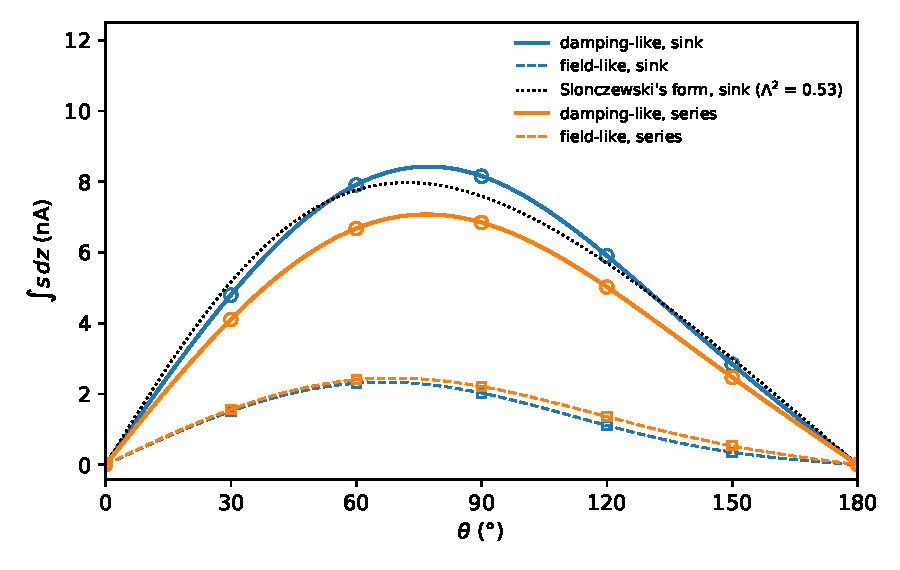
\includegraphics[width=0.85\textwidth]{slonczewski_angle_torque.pdf}
\caption{Accumulations damping-like ($\int s_y\,dz$, traits pleins et
  cercles) et field-like ($\int s_x\,dz$, tirets et carrés) intégrées sur
  l'épaisseur de F2 : référence (traits) et FeeLLGood (symboles), modèles
  \texttt{sink} et \texttt{series}. Pointillés : forme de Slonczewski
  ajustée sur le couple damping-like (\texttt{sink}).}
\label{fig:couple}
\end{figure}

La figure~\ref{fig:couple} et les tables ci-dessous donnent les
accumulations intégrées sur l'épaisseur (en A), qui mesurent les couples.
À 0 et $180^\circ$, l'accumulation transverse est nulle.

\begin{center}
\small
\renewcommand{\arraystretch}{1.15}
\begin{tabular}{rccc}
  \toprule
  \multicolumn{4}{c}{\texttt{transverse: sink} (par défaut)} \\
  $\theta$ & damping-like $\int s_y\,dz$ & field-like $\int s_x\,dz$ & erreur max \\
  & FeeLLGood / réf ($10^{-9}$\,A) & FeeLLGood / réf ($10^{-9}$\,A) & sur $\vs$ \\
  \midrule
  30  & 4.7941 / 4.7930 & 1.5079 / 1.5266 & $4.6\times10^{-3}$ \\
  60  & 7.9075 / 7.9065 & 2.2985 / 2.3291 & $1.1\times10^{-2}$ \\
  90  & 8.1529 / 8.1531 & 2.0235 / 2.0547 & $5.2\times10^{-3}$ \\
  120 & 5.9018 / 5.9031 & 1.1078 / 1.1300 & $2.3\times10^{-3}$ \\
  150 & 2.8398 / 2.8410 & 0.35261 / 0.36310 & $1.0\times10^{-3}$ \\
  \midrule
  \multicolumn{4}{c}{\texttt{transverse: series}} \\
  \midrule
  30  & 4.1054 / 4.1033 & 1.5626 / 1.5755 & $4.1\times10^{-3}$ \\
  60  & 6.6736 / 6.6702 & 2.4030 / 2.4238 & $1.1\times10^{-2}$ \\
  90  & 6.8434 / 6.8403 & 2.2136 / 2.2346 & $4.6\times10^{-3}$ \\
  120 & 5.0217 / 5.0198 & 1.3620 / 1.3772 & $1.9\times10^{-3}$ \\
  150 & 2.4700 / 2.4694 & 0.53402 / 0.54143 & $7.6\times10^{-4}$ \\
  \bottomrule
\end{tabular}
\end{center}
L'erreur maximale sur $\vs$, rapportée à $\max|\vs|$, reste inférieure à
$1.2\times10^{-2}$. L'accumulation damping-like est reproduite à quelques
$10^{-4}$ près, la field-like à 1 à 3\,\% : $s_x$ change de signe dans
l'épaisseur (figure~\ref{fig:profil}), et son intégrale résulte d'une
compensation, qui amplifie l'erreur relative.

\subsection{Profils}

\begin{figure}[h]
\centering
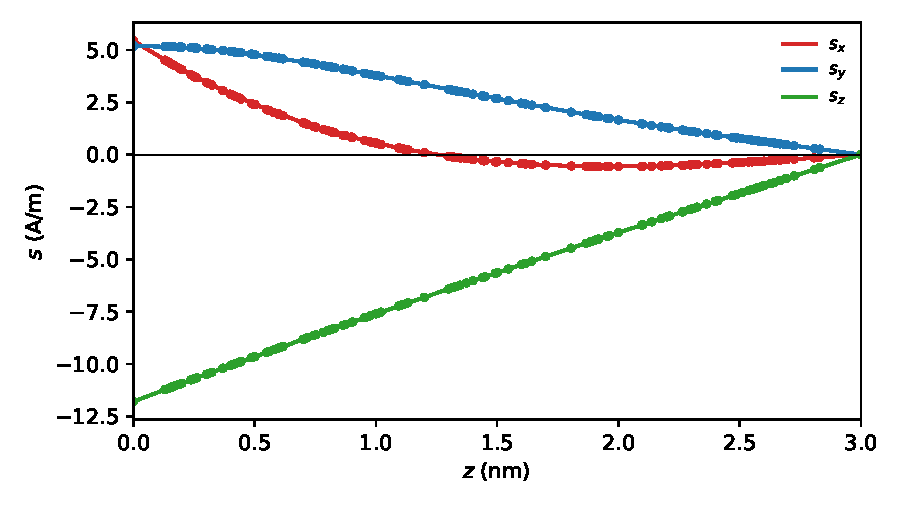
\includegraphics[width=0.8\textwidth]{slonczewski_angle_profile.pdf}
\caption{Composantes de $\vs$ dans l'épaisseur de F2 à $\theta = 90^\circ$
  (\texttt{sink}) : référence (traits) et FeeLLGood en 200 nœuds tirés au
  hasard (cercles).}
\label{fig:profil}
\end{figure}

La figure~\ref{fig:profil} montre les trois composantes à $\theta =
90^\circ$. Le courant transverse entre polarisé surtout selon $x$ : $s_x$
est maximal à l'entrée, puis tourne vers $y$ et change de signe vers
1.2\,nm, comme le prévoit $\kappa$. $s_y$ décroît presque linéairement
jusqu'au réservoir de sortie. L'accumulation longitudinale $s_z$ est
négative : à $90^\circ$, le courant entre dans F2 moins polarisé selon
$\vm$ que F2 ne le transporte en volume.

\subsection{Convergence et sensibilité}

L'erreur décroît comme $h^2$ ($1.1\times10^{-2}$ à $h = 0.2$\,nm,
$2.7\times10^{-3}$ à $h = 0.1$\,nm, vérifié avec \texttt{series} et
$\mathrm{Im}\,G_{\uparrow\downarrow} = 0$). Le test échoue (tolérance
2\,\%) si :
\begin{itemize}
  \item la conversion est $k\,G_{\uparrow\downarrow}$ au lieu de
    $2k\,G_{\uparrow\downarrow}$ (\texttt{series},
    $\mathrm{Im}\,G_{\uparrow\downarrow} = 0$) : erreur de 170\,\% ;
  \item le signe du terme en $\mathrm{Im}\,G_{\uparrow\downarrow}$ de la
    référence est inversé (\texttt{IM\_SIGN = -1}, \texttt{series}) :
    erreur de 13\,\%, l'accumulation field-like différant d'un facteur 2 à
    $150^\circ$ ;
  \item le modèle de la référence n'est pas celui de FeeLLGood : les deux
    modèles diffèrent de 15 à 17\,\% sur le couple damping-like.
\end{itemize}

\subsection{Utilisation}

\begin{verbatim}
cd validation/slonczewski_angle
./slonczewski_angle.py [chemin de feellgood]   # défaut : ../../src/feellgood
./plot_figures.py                              # figures de ce document
\end{verbatim}
Le maillage est construit par \texttt{gmsh} s'il manque. Le script lance
FeeLLGood pour chaque modèle et chaque angle (14 calculs, environ 20\,s),
affiche pour chaque angle les intégrales ci-dessus et l'erreur maximale,
puis l'ajustement à la forme de Slonczewski :
\begin{verbatim}
damping-like torque (reference): Lambda^2 = 0.5315,
    deviation from the form of Slonczewski 5.2e-02
\end{verbatim}
Le code de retour est 0 si l'erreur est inférieure à 2\,\% à tous les
angles.

\section{Limites du test}

\begin{itemize}
  \item F1 est un réservoir idéal : la renormalisation par le volume de F1
    est vérifiée par \texttt{valet\_fert\_1d}.
  \item L'aimantation de F2 est uniforme et fixe : le couplage avec LLG,
    le couple agissant sur une aimantation qui bouge, est montré par
    l'exemple \texttt{examples/}\allowbreak\texttt{pillar\_slonczewski\_}\allowbreak
    \texttt{current\_density\_ramp1ns}.
  \item Toutes les régions ont la même densité d'états : voir
    \texttt{validation/two\_regions\_1d}.
  \item Le test ne dit pas lequel de \texttt{sink} et \texttt{series} est
    physiquement juste : cela dépend de ce que contient le
    $G_{\uparrow\downarrow}$ donné (toute l'absorption, ou la seule part
    de l'interface).
\end{itemize}

\section*{Références}

\begin{itemize}
  \item J.\,C.~Slonczewski, J.~Magn.\ Magn.\ Mater.\ \textbf{159}, L1
    (1996) ; \textbf{247}, 324 (2002) : couple de transfert de spin,
    dépendance angulaire à paramètre $\Lambda$.
  \item A.~Brataas, G.\,E.\,W.~Bauer, P.\,J.~Kelly, Phys.\ Rep.\
    \textbf{427}, 157 (2006) : théorie des circuits magnéto-électroniques,
    conductance de mélange.
  \item T.~Valet, A.~Fert, Phys.\ Rev.\ B \textbf{48}, 7099 (1993).
  \item S.~Zhang, P.\,M.~Levy, A.~Fert, Phys.\ Rev.\ Lett.\ \textbf{88},
    236601 (2002) : diffusion de spin non colinéaire.
  \item C.~Petitjean, D.~Luc, X.~Waintal, Phys.\ Rev.\ Lett.\
    \textbf{109}, 117204 (2012) : courants de spin transverses en
    dérive--diffusion, conditions d'interface cohérentes.
  \item V.~Baltz, \emph{The Basics of Electron Transport in Spintronics},
    EDP Sciences (2023), §4.2--4.6.
  \item \texttt{validation/valet\_fert\_1d/valet\_fert\_1d\_french.tex} :
    le test colinéaire, le modèle de Valet--Fert et la conversion
    $\vs = \mu_BN_0e\vphi/2$.
  \item \texttt{dev-notes/slonczewski\_polarisation.tex} : dérivation
    détaillée de la condition de Robin.
  \item \texttt{dev-notes/spin\_injection\_boundary\_conditions.md} (en
    anglais) : la même, avec la mise en œuvre dans FeeLLGood.
\end{itemize}

\end{document}
